\section{Split-DASH System Architecture}
The DASH or DASH like system provides a way (guideline) to change video quality instead of pausing a video streaming during bad network quality. There are several implementation of the DASH or DASH like streaming system and most of them have a HTML5 based implementation using {\it Media Source Extension}(MSE)\cite{wiki:dash,w3c:mse}. These implementations also support {\it Digital Right Management}(DRM) via {\it Encrypted Media Extension}(EME)\cite{w3c:eme}. These implementation have several modules implemented either in {\it Javascript} or in browser. The modules like playback, media decryption are implemented in browser or some browser extension/plugin (\ie Widevine plugin for DRM protection). The different modules are as follows:

{\bf Playback module} or the player is the module which actually render the video. It is implemented mostly in the browser. It is mostly implemented in the browser and render in a html element. The player is accessed and controlled via MSE APIs.

{\bf Buffer controller} manages and monitor video buffer. It is partly implemented using javascript and partly by the browser itself.

{\bf Adaptive bitrate controller} is the module decides the quality based on the network condition. It can have multiple algorithm and implemented in javascript it self. It is the most crucial part of DASH like streaming system yet the most flexible part. Any streaming provider can implement there won algorithm based on their requirement. We will discuss more about ABR later part of the article.

{\bf Download manager} is responsible for downloading the segment/chunk chosen by the ABR algorithm. It monitors the progress of ongoing downloads to gain fine tune information about the network condition. Most of the time it download chunk using AJAX (Asynchronous JavaScript And XML)


{\bf CDN/Streaming Servers} are http based static file server. It contains all the data requires to play a video smoothly.

{\bf DRM protection module:} It provides DRM protection using EME when a streaming provider wants to protect the right of content. It is an independent component and does not influence the ABR algorithm or other components. DRM protection module is out of the scope of this work.

\begin{figure}[ht]
   \begin{center}
           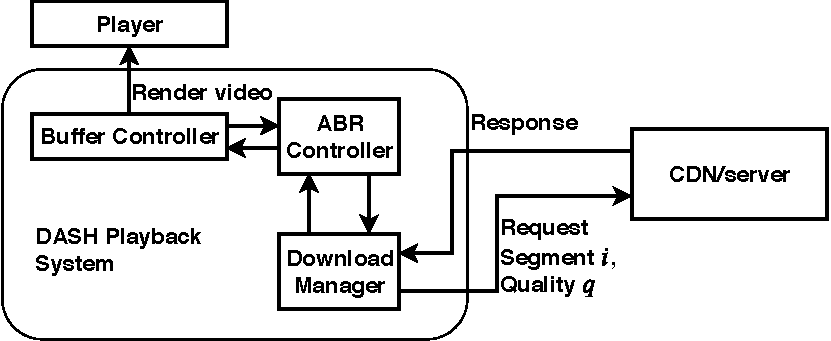
\includegraphics[width=0.7\linewidth]{img/playerDiagram_basic}
   \end{center}
   \caption{\label{fig:playerDiagram_basic} Average bitrate variation during playback}
\end{figure}

The inter-connection of the modules are depicted in the Fig.~\ref{fig:playerDiagram_basic}. Here, the ABR controller controls the playback via buffer controller while instructing download manager to download appropriate segment in the appropriate time. The ABR controller is the most important component. There are active research going on to improve ABR controller. As ABR controller is the part of the player, it need to be implemented in client application it self. In case HTML based player, ABRs need to be implemented in javascript. The ABR algorithm like MPC\cite{dash:mpc}, BOLA\cite{dash:bola} or the alogorithms described in \cite{dash:probe,dash:cs2p,dash:CFA,dash:rnb,dash:buffer} does not have any special library requirement and can be implemented easily in any technology. However, as machine learning based ABR algorithm like Pensieve\cite{dash:pensieve}, OBOE\cite{dash:oboe} or HotDASH\cite{dash:hotdash} need specialized machine learning (ML) library and very hard to implement if the technology does not have support for required library. So, it is very difficult to deploy these algorithm in browser based video player.

Authors of the ML based algorithm show prototype by modifying the system little bit. The new architecture looks like Fig.~[ref].